\documentclass[a4paper]{article}
\usepackage{student}

% PREENCHA ESSA PARTE COM SEUS DADOS

\setuniversity{UNIVERSIDADE DO ESTADO DE SANTA CATARINA}
\setdepartment{CENTRO DE EDUCAÇÃO DO PLANALTO NORTE/DEPARTAMENTO DE SISTEMAS DE INFORMAÇÃO}
\setmodule{ROTEIRO DE ATIVIDADES ESP-32 e IoT}
\setterm{2025/5° FASE}

\title{AUTOMAÇÃO DE SISTEMAS}
\setmembername{LISTA DE NOMES DOS ALUNOS}
\setmemberuid{LISTA DE MATRÍCULAS DOS ALUNOS}

\usepackage{amsmath,amssymb,bm}
\usepackage{hyperref}


\begin{document}

    \header{}
    % UTILIZAR O AMBIENTE "answer" para criar uma nova caixa de resposta
    % O texto entre chaves [] será utilizado como título antes da caixa
    % Exemplo abaixo:
    
    \begin{answer}[1. Introdução ao ESP32 e Conceitos de IoT]
    \begin{enumerate}
        \item O que é o microcontrolador?
         
            Um microcontrolador é um circuito integrado que contém um processador, 
            memória e periféricos de entrada/saída em um único chip, sendo utilizado
            para controlar dispositivos eletrônicos de forma autônoma.

        \item Diferença entre ESP8266, ESP32 e Arduino Uno.
        
            O ESP8266 é um microcontrolador com conectividade Wi-Fi, enquanto o ESP32
            é uma versão mais avançada com Wi-Fi e Bluetooth integrados, oferecendo
            mais recursos e potência de processamento. O Arduino Uno é uma placa
            de prototipagem baseada no microcontrolador ATmega328, que não possui
            conectividade Wi-Fi ou Bluetooth nativa, mas é amplamente utilizado
            para projetos de eletrônica e programação básica.

        \item Conceitos básicos de Internet das Coisas (IoT).
        
            Internet das Coisas (IoT) refere-se à interconexão de dispositivos físicos
            à internet, permitindo que eles coletem e compartilhem dados, além de
            serem controlados remotamente. Isso possibilita a automação, monitoramento
            e otimização de processos em diversas áreas, como residências, indústrias
            e cidades inteligentes.
        
        \item Exemplos de aplicações com ESP32 e IoT.
            O ESP32 pode ser utilizado em diversas aplicações de IoT, como:

            \begin{itemize}
                \item Monitoramento ambiental (temperatura, umidade, qualidade do ar);
                \item Automação residencial (controle de luzes, eletrodomésticos, sistemas de segurança);
                \item Sistemas de irrigação inteligente;
                \item Dispositivos vestíveis (wearables) para monitoramento de saúde;
                \item Controle remoto de robôs e drones.
            \end{itemize}
    \end{enumerate}
    \end{answer}
    
    \begin{answer}[2. Instalação da IDE Arduino e Configuração do ESP32.]
        \begin{enumerate}
            \item  Instalação da IDE Arduino:

                A IDE Arduino é uma plataforma de desenvolvimento integrada que permite
                programar microcontroladores, incluindo o ESP32. Para instalar a IDE,
                basta baixar o instalador do site oficial do Arduino e seguir as instruções
                de instalação.

                \begin{itemize}
                    \item  Acesse o site oficial do Arduino: \url{https://www.arduino.cc/en/software}.
                    \item  Baixe a versão adequada para o seu sistema operacional (Windows, macOS, Linux).
                    \item  Execute o instalador e siga as instruções na tela.
                    \item  Após a instalação, abra a IDE Arduino.
                \end{itemize}
            \item Configuração do ESP32 na IDE Arduino:
            
                Para programar o ESP32 na IDE Arduino, é necessário instalar o suporte
                ao ESP32. Siga os passos abaixo:

                \begin{itemize}
                    \item  Abra a IDE Arduino.
                    \item  Vá para "File" $>$ "Preferences".
                    \item  Na seção "Additional Boards Manager URLs", adicione a seguinte  URL:
                        \url{https://raw.githubusercontent.com/espressif/arduino-esp32/gh-pages/package_esp32_index.json}.
                    \item  Para facilitar, veja a imagem abaixo mostrando onde adicionar a URL:

                        \begin{center}
                            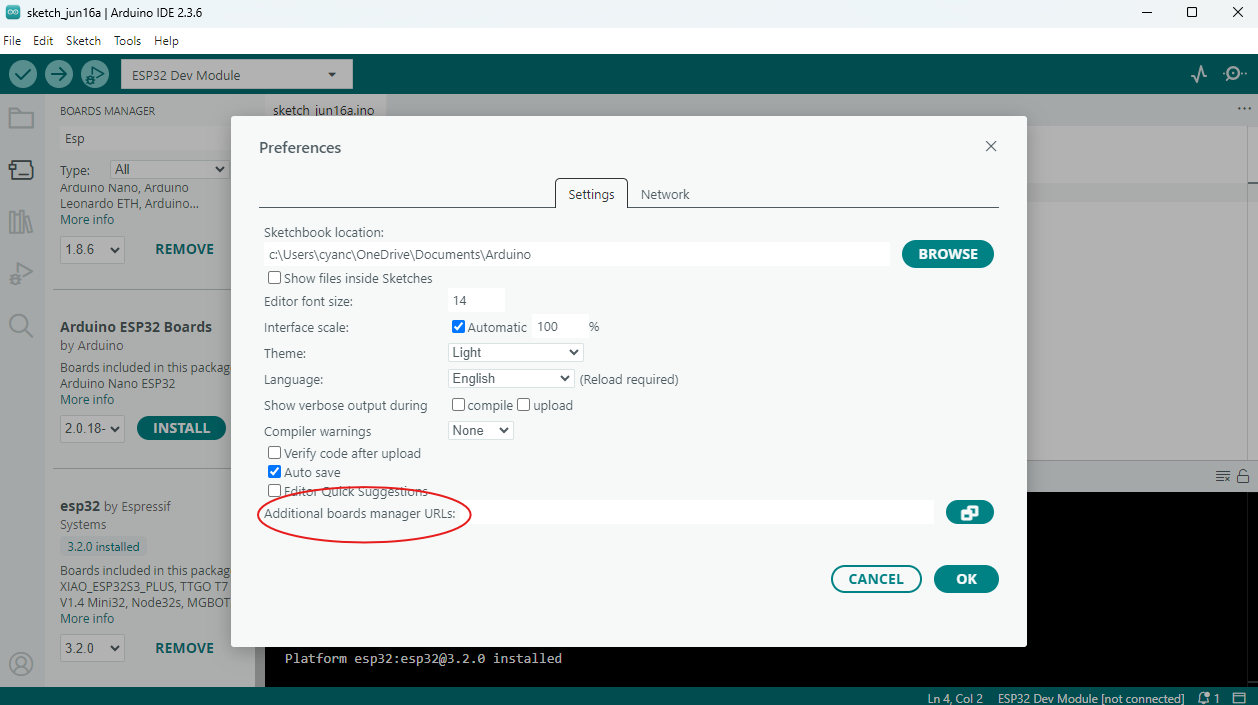
\includegraphics[width=0.7\textwidth]{images/addURL}
                        \end{center}
                    \item  Clique em "OK" para salvar as preferências.
                    \item  Vá para "Tools" $>$ "Board" $>$ "Boards Manager".
                    \item  Pesquise por "ESP32" e instale o pacote "esp32 by Espressif".
                    \item  Veja a imagem abaixo mostrando a seleção da placa:

                        \begin{center}
                            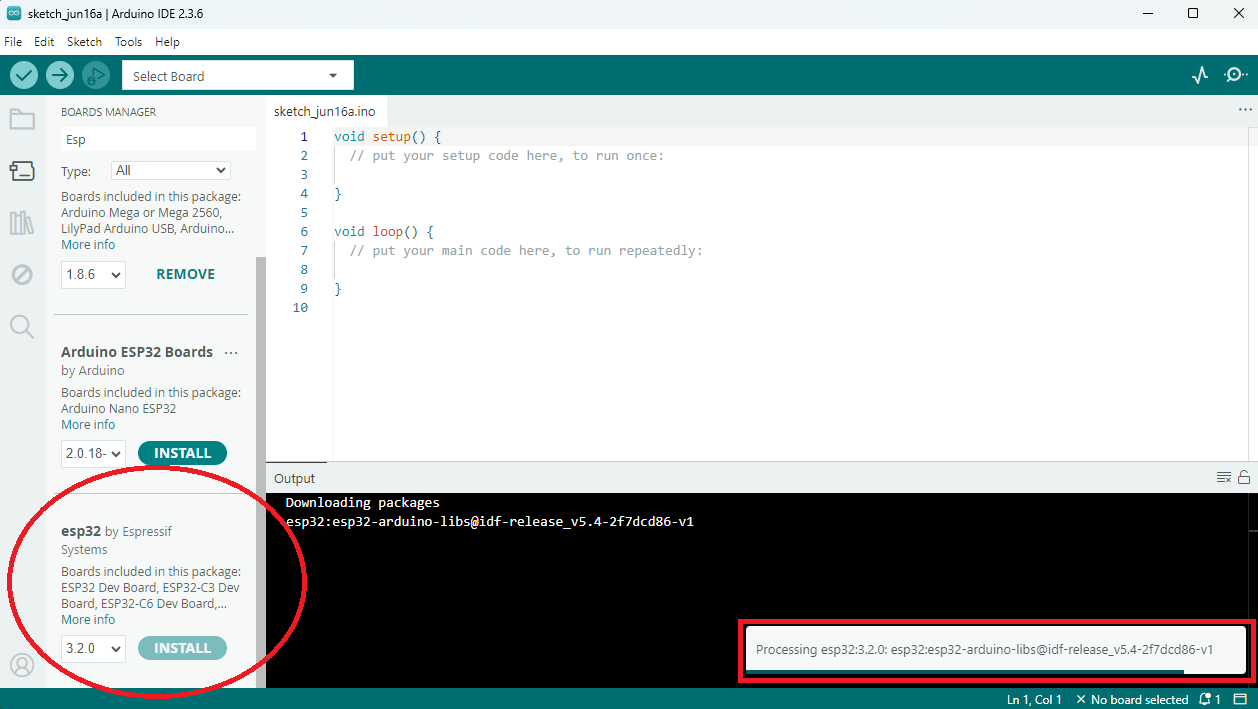
\includegraphics[width=0.7\textwidth]{images/Esp-32-board-install.png}
                        \end{center}
                    \item  Após a instalação, selecione a sua placa ESP32 em "Tools" $>$ "Board".
                    \item  Após instalar o pacote e selecionr a placa, conecte sua placa ESP32 ao computador.
                    \item  Selecione a porta correta em "Tools" $>$ "Port".
                    
                \end{itemize}
            \item  Teste de conexão com código "Blink":

                Para verificar se a configuração está correta, você pode carregar o
                exemplo "Blink" na IDE Arduino. Siga os passos abaixo:

                \begin{itemize}
                    \item  Vá para "File" $>$ "Examples" $>$ "01.Basics" $>$ "Blink".
                    \item  O código do exemplo deve ser semelhante ao seguinte:

                    \begin{verbatim}
                    void setup() {
                        pinMode(LED_BUILTIN, OUTPUT);
                    }

                    void loop() {
                        digitalWrite(LED_BUILTIN, HIGH); // Liga LED
                        delay(1000); // Espera por 1 segundo
                        digitalWrite(LED_BUILTIN, LOW); // Desliga LED
                        delay(1000); // Espera por 1 segundo
                    }
                    \end{verbatim}

                    \item  Carregue o código na placa ESP32 clicando no botão de upload (seta para a direita).
                    \begin{center}
                        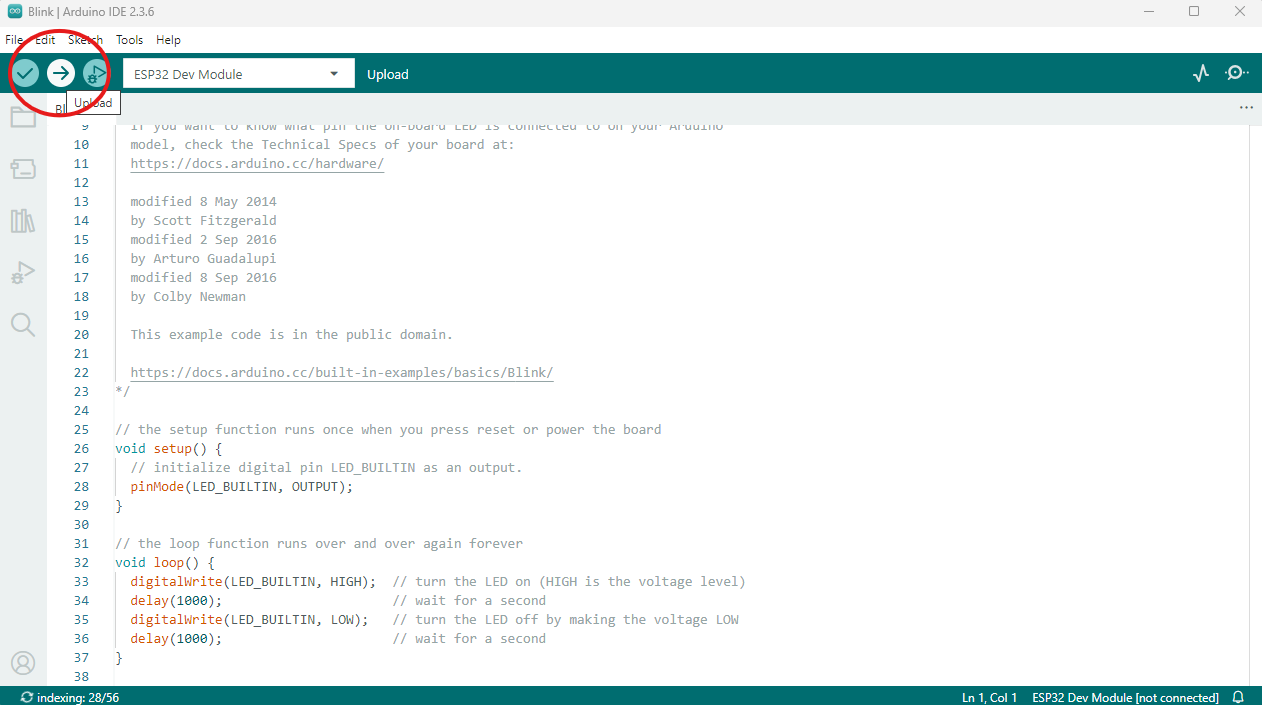
\includegraphics[width=0.7\textwidth]{images/upload.png}
                    \end{center}
                    \item  Após o upload, o LED integrado da placa deve piscar a cada segundo.
                \end{itemize}
        \end{enumerate}
    \end{answer}

    \begin{answer}[3. Comparação com ESP8266 e Arduino Uno.]
        \begin{itemize}
            \item \textbf{ESP32:} Microcontrolador avançado da Espressif, possui processador dual-core, conectividade Wi-Fi e Bluetooth integrados, maior quantidade de pinos de entrada/saída, suporte a múltiplos periféricos, ADCs de maior resolução e maior capacidade de processamento e memória. Ideal para aplicações IoT mais complexas e que exigem conectividade sem fio diversificada.
            \item \textbf{ESP8266:} Também da Espressif, é mais simples que o ESP32, com processador single-core, conectividade Wi-Fi integrada, menos pinos e recursos. É indicado para projetos IoT básicos que demandam apenas Wi-Fi e menor consumo de recursos.
            \item \textbf{Arduino Uno:} Baseado no microcontrolador ATmega328P, não possui conectividade Wi-Fi ou Bluetooth nativa, mas é muito utilizado em projetos de eletrônica básica, prototipagem e ensino. Possui menos memória e processamento em relação aos ESPs, mas conta com vasta documentação e comunidade.
        \end{itemize}

        \textbf{Resumo:} O ESP32 é o mais completo em termos de recursos e conectividade, seguido pelo ESP8266 (mais simples e barato), enquanto o Arduino Uno é ideal para projetos básicos sem necessidade de conexão sem fio.
    \end{answer}

    \begin{answer}[4. Leitura de sensores analógicos e digitais]

        Obetivo: Aprender a ler dados de sensores analógicos e digitais utilizando o ESP32.
        \begin{enumerate}
            \item Leitura de sensores analógicos:

                Para ler dados de sensores analógicos, como um potenciômetro ou sensor de temperatura, você pode usar a função `analogRead()`. O ESP32 possui vários pinos ADC (Conversores Analógico-Digital) que podem ser utilizados para essa finalidade.

                Exemplo de código para ler um sensor analógico:

            \begin{verbatim}
            int sensorPin = 34; // Pino ADC
            int sensorValue = 0;

            void setup() {
                Serial.begin(115200);
            }

            void loop() {
                sensorValue = analogRead(sensorPin); // Lê o valor do sensor
                Serial.println(sensorValue); // Imprime o valor no monitor serial
                delay(1000); // Espera 1 segundo
            }
            \end{verbatim}

            \item Leitura de sensores digitais:

                Para ler dados de sensores digitais, como um botão ou sensor de movimento, você pode usar a função `digitalRead()`. O ESP32 possui vários pinos digitais que podem ser utilizados para essa finalidade.

                Exemplo de código para ler um sensor digital:

            \begin{verbatim}
            int buttonPin = 2; // Pino digital
            int buttonState = 0;

            void setup() {
                pinMode(buttonPin, INPUT); // Configura o pino como entrada
                Serial.begin(115200);
            }

            void loop() {
                buttonState = digitalRead(buttonPin); // Lê o estado do botão
                Serial.println(buttonState); // Imprime o estado no monitor serial
                delay(1000); // Espera 1 segundo
            }
            \end{verbatim}
        \end{enumerate}
    \end{answer}

    \begin{answer}[5. Controle de atuadores (EX: LED e buzzer).]
        \begin{enumerate}
            \item Controle de LED:

                Para controlar um LED, você pode usar a função `digitalWrite()`. O ESP32 possui vários pinos digitais que podem ser utilizados para essa finalidade.

                Exemplo de código para controlar um LED:

            \begin{verbatim}
            int ledPin = 2; // Pino do LED

            void setup() {
                pinMode(ledPin, OUTPUT); // Configura o pino como saída
            }

            void loop() {
                digitalWrite(ledPin, HIGH); // Liga o LED
                delay(1000); // Espera 1 segundo
                digitalWrite(ledPin, LOW); // Desliga o LED
                delay(1000); // Espera 1 segundo
            }
            \end{verbatim}

            \item Controle de buzzer:

                Para controlar um buzzer, você também pode usar a função `digitalWrite()`.

                Exemplo de código para controlar um buzzer:

            \begin{verbatim}
            int buzzerPin = 2; // Pino do buzzer

            void setup() {
                pinMode(buzzerPin, OUTPUT); // Configura o pino como saída
            }

            void loop() {
                // Aumenta a frequência gradualmente (efeito de sirene)
                for (int freq = 800; freq <= 2000; freq += 10) {
                    tone(buzzerPin, freq); // Gera tom com a frequência atual
                    delay(10); // Pequeno atraso para suavizar a transição
                }
                
                // Diminui a frequência gradualmente
                for (int freq = 2000; freq >= 800; freq -= 10) {
                    tone(buzzerPin, freq); // Gera tom com a frequência atual
                    delay(10); // Pequeno atraso para suavizar a transição
                }
                
                noTone(buzzerPin); // Para o som
                delay(200); // Pausa breve antes de reiniciar
                }
            \end{verbatim}
        \end{enumerate}
    \end{answer}

    \begin{answer}[6. Conectando o ESP32 a uma rede Wi-Fi.]
        Quisque eget velit eget arcu rhoncus dictum non quis turpis. Nulla fermentum nulla nec vestibulum lacinia. Sed aliquam euismod dolor a efficitur. Fusce a nisi at justo vulputate tempor sed id lectus. Vestibulum ante ipsum primis in faucibus orci luctus et ultrices posuere cubilia curae; Duis imperdiet ut dolor at varius. Pellentesque mattis turpis diam, et maximus orci aliquet id. Sed luctus a magna ac mattis. Sed ultricies quis turpis nec consequat. Donec a placerat metus, a tempor nulla. Maecenas gravida, diam sed aliquet efficitur, magna risus pulvinar orci, vel rutrum velit metus et tortor. Nam maximus, nulla eu semper scelerisque, mi sem vulputate tellus, nec hendrerit nulla ligula vel libero. Maecenas convallis pellentesque massa a ornare.

        Nam rhoncus magna sit amet porttitor condimentum. Vestibulum rhoncus consectetur est nec volutpat. Mauris volutpat nisi at tortor auctor, id ornare eros tempus. Aliquam et sapien mattis, eleifend turpis et, bibendum ipsum. Quisque vel semper risus, nec aliquam dolor. Maecenas non semper risus, sagittis eleifend nunc. Cras turpis elit, vulputate in porttitor at, rutrum eget justo. Orci varius natoque penatibus et magnis dis parturient montes, nascetur ridiculus mus. Cras quis placerat tellus, eget gravida nunc. Integer malesuada vitae tortor non sollicitudin. Suspendisse eu sem purus.
    \end{answer}

    \begin{answer}[7. Introdução ao protocolo MQTT.]
        Quisque eget velit eget arcu rhoncus dictum non quis turpis. Nulla fermentum nulla nec vestibulum lacinia. Sed aliquam euismod dolor a efficitur. Fusce a nisi at justo vulputate tempor sed id lectus. Vestibulum ante ipsum primis in faucibus orci luctus et ultrices posuere cubilia curae; Duis imperdiet ut dolor at varius. Pellentesque mattis turpis diam, et maximus orci aliquet id. Sed luctus a magna ac mattis. Sed ultricies quis turpis nec consequat. Donec a placerat metus, a tempor nulla. Maecenas gravida, diam sed aliquet efficitur, magna risus pulvinar orci, vel rutrum velit metus et tortor. Nam maximus, nulla eu semper scelerisque, mi sem vulputate tellus, nec hendrerit nulla ligula vel libero. Maecenas convallis pellentesque massa a ornare.

        Nam rhoncus magna sit amet porttitor condimentum. Vestibulum rhoncus consectetur est nec volutpat. Mauris volutpat nisi at tortor auctor, id ornare eros tempus. Aliquam et sapien mattis, eleifend turpis et, bibendum ipsum. Quisque vel semper risus, nec aliquam dolor. Maecenas non semper risus, sagittis eleifend nunc. Cras turpis elit, vulputate in porttitor at, rutrum eget justo. Orci varius natoque penatibus et magnis dis parturient montes, nascetur ridiculus mus. Cras quis placerat tellus, eget gravida nunc. Integer malesuada vitae tortor non sollicitudin. Suspendisse eu sem purus.
    \end{answer}

    \begin{answer}[8. Publicando dados do sensor em um broker MQTT.]
        Quisque eget velit eget arcu rhoncus dictum non quis turpis. Nulla fermentum nulla nec vestibulum lacinia. Sed aliquam euismod dolor a efficitur. Fusce a nisi at justo vulputate tempor sed id lectus. Vestibulum ante ipsum primis in faucibus orci luctus et ultrices posuere cubilia curae; Duis imperdiet ut dolor at varius. Pellentesque mattis turpis diam, et maximus orci aliquet id. Sed luctus a magna ac mattis. Sed ultricies quis turpis nec consequat. Donec a placerat metus, a tempor nulla. Maecenas gravida, diam sed aliquet efficitur, magna risus pulvinar orci, vel rutrum velit metus et tortor. Nam maximus, nulla eu semper scelerisque, mi sem vulputate tellus, nec hendrerit nulla ligula vel libero. Maecenas convallis pellentesque massa a ornare.

        Nam rhoncus magna sit amet porttitor condimentum. Vestibulum rhoncus consectetur est nec volutpat. Mauris volutpat nisi at tortor auctor, id ornare eros tempus. Aliquam et sapien mattis, eleifend turpis et, bibendum ipsum. Quisque vel semper risus, nec aliquam dolor. Maecenas non semper risus, sagittis eleifend nunc. Cras turpis elit, vulputate in porttitor at, rutrum eget justo. Orci varius natoque penatibus et magnis dis parturient montes, nascetur ridiculus mus. Cras quis placerat tellus, eget gravida nunc. Integer malesuada vitae tortor non sollicitudin. Suspendisse eu sem purus.
    \end{answer}

    \begin{answer}[9. Recebendo comandos MQTT para controle de atuadores.]
        Quisque eget velit eget arcu rhoncus dictum non quis turpis. Nulla fermentum nulla nec vestibulum lacinia. Sed aliquam euismod dolor a efficitur. Fusce a nisi at justo vulputate tempor sed id lectus. Vestibulum ante ipsum primis in faucibus orci luctus et ultrices posuere cubilia curae; Duis imperdiet ut dolor at varius. Pellentesque mattis turpis diam, et maximus orci aliquet id. Sed luctus a magna ac mattis. Sed ultricies quis turpis nec consequat. Donec a placerat metus, a tempor nulla. Maecenas gravida, diam sed aliquet efficitur, magna risus pulvinar orci, vel rutrum velit metus et tortor. Nam maximus, nulla eu semper scelerisque, mi sem vulputate tellus, nec hendrerit nulla ligula vel libero. Maecenas convallis pellentesque massa a ornare.

        Nam rhoncus magna sit amet porttitor condimentum. Vestibulum rhoncus consectetur est nec volutpat. Mauris volutpat nisi at tortor auctor, id ornare eros tempus. Aliquam et sapien mattis, eleifend turpis et, bibendum ipsum. Quisque vel semper risus, nec aliquam dolor. Maecenas non semper risus, sagittis eleifend nunc. Cras turpis elit, vulputate in porttitor at, rutrum eget justo. Orci varius natoque penatibus et magnis dis parturient montes, nascetur ridiculus mus. Cras quis placerat tellus, eget gravida nunc. Integer malesuada vitae tortor non sollicitudin. Suspendisse eu sem purus.
    \end{answer}

    \begin{answer}[10. Projeto Final – Estação IoT com sensor + LED.]
        Quisque eget velit eget arcu rhoncus dictum non quis turpis. Nulla fermentum nulla nec vestibulum lacinia. Sed aliquam euismod dolor a efficitur. Fusce a nisi at justo vulputate tempor sed id lectus. Vestibulum ante ipsum primis in faucibus orci luctus et ultrices posuere cubilia curae; Duis imperdiet ut dolor at varius. Pellentesque mattis turpis diam, et maximus orci aliquet id. Sed luctus a magna ac mattis. Sed ultricies quis turpis nec consequat. Donec a placerat metus, a tempor nulla. Maecenas gravida, diam sed aliquet efficitur, magna risus pulvinar orci, vel rutrum velit metus et tortor. Nam maximus, nulla eu semper scelerisque, mi sem vulputate tellus, nec hendrerit nulla ligula vel libero. Maecenas convallis pellentesque massa a ornare.

        Nam rhoncus magna sit amet porttitor condimentum. Vestibulum rhoncus consectetur est nec volutpat. Mauris volutpat nisi at tortor auctor, id ornare eros tempus. Aliquam et sapien mattis, eleifend turpis et, bibendum ipsum. Quisque vel semper risus, nec aliquam dolor. Maecenas non semper risus, sagittis eleifend nunc. Cras turpis elit, vulputate in porttitor at, rutrum eget justo. Orci varius natoque penatibus et magnis dis parturient montes, nascetur ridiculus mus. Cras quis placerat tellus, eget gravida nunc. Integer malesuada vitae tortor non sollicitudin. Suspendisse eu sem purus.
    \end{answer}

    \begin{answer}[11. Encerramento e Discussão de Aplicações Reais.]
        //aqui eu faço depois
    \end{answer}

\end{document}
